\documentclass[DIN, pagenumber=false, fontsize=11pt, parskip=half]{scrartcl}

\usepackage{amsmath}
\usepackage{amsfonts}
\usepackage{amssymb}
\usepackage{enumitem}
\usepackage[utf8]{inputenc} % this is needed for umlauts
\usepackage[ngerman]{babel} % this is needed for umlauts
\usepackage[T1]{fontenc} 
\usepackage{commath}
\usepackage{xcolor}
\usepackage{booktabs}
\usepackage{float}
\usepackage{tikz-timing}
\usepackage{tikz}

\usetikzlibrary{calc,shapes.multipart,chains,arrows}

\title{Grundlagen der Betriebssysteme}
\author{Tim Luchterhand, Paul Nykiel (Gruppe 017)}

\begin{document}
    \maketitle
    \section{Freispeichervergabe}
    \subsection{}
    \begin{equation*}
        1 \text{KiB} = 1024 \text{Bytes}
    \end{equation*}

    \subsection{}
    \begin{enumerate}[label=\Alph*]
        \item 2 Blöcke
        \item 2 Blöcke
        \item 1 Block
        \item 3 Blöcke
        \item 1 Block
    \end{enumerate}

    \subsection{}
    Speicherblock A in \textcolor{red}{rot}, Speicherblock B in \textcolor{green}{grün}, Speicherblock C in \textcolor{blue}{blau},
    Speicherblock D in \textcolor{yellow}{gelb} und Speicherblock E in \textcolor{purple}{lila}.
    \subsubsection{First Fit}
    \begin{figure}[H]
        \centering
        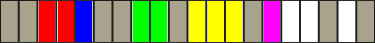
\includegraphics[width=\textwidth]{firstFit.png}
        \caption{Speicheraufteilung nach First-Fit}
    \end{figure}
    \subsubsection{Next Fit}
    \begin{figure}[H]
        \centering
        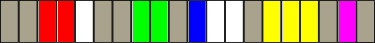
\includegraphics[width=\textwidth]{nextFit.png}
        \caption{Speicheraufteilung nach Next-Fit}
    \end{figure}
    \subsubsection{Best Fit}
    \begin{figure}[H]
        \centering
        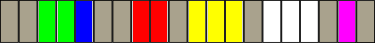
\includegraphics[width=\textwidth]{bestFit.png}
        \caption{Speicheraufteilung nach Best-Fit}
    \end{figure}
    \subsubsection{Worst Fit}
    Der Speicherblock D konnte nicht untergebracht werden.
    \begin{figure}[H]
        \centering
        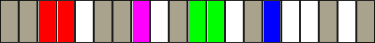
\includegraphics[width=\textwidth]{worstFit.png}
        \caption{Speicheraufteilung nach Worst-Fit}
    \end{figure}

    \section{Getrennte Listen}
    \subsection{}
    \begin{figure}[H]
        \centering
        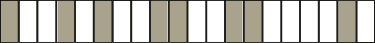
\includegraphics[width=\textwidth]{freiSpeicher.png}
        \caption{Speicher mit Blöcken je 4 Bytes}
    \end{figure}
    \begin{figure}[H]
        \centering
        \begin{tikzpicture}[draw, minimum width=1cm, minimum height=0.5cm]
            \node[draw, text width=1.5cm] (s1) at (0, 0) {Addr: 1\\Size: 2};
            \node[draw, text width=1.5cm] (s2) at (2, 0) {Addr: 4\\Size: 1};
            \node[draw, text width=1.5cm] (s3) at (4, 0) {Addr: 6\\Size: 2};
            \node[draw, text width=1.5cm] (s4) at (6, 0) {Addr: 10\\Size: 2};
            \node[draw, text width=1.5cm] (s5) at (8, 0) {Addr: 14\\Size: 4};
            \node[draw, text width=1.5cm] (s6) at (10, 0) {Addr: 19\\Size: 1};

            \draw[->] (s1) -- (s2);
            \draw[->] (s2) -- (s3);
            \draw[->] (s3) -- (s4);
            \draw[->] (s4) -- (s5);
            \draw[->] (s5) -- (s6);
        \end{tikzpicture}
        \caption{Freispeicherliste}
    \end{figure}
    \begin{figure}[H]
        \centering
        \begin{tikzpicture}[draw, minimum width=1cm, minimum height=0.5cm]
            \node[draw] (b1) at (0,0) {Size: 1};
            \node[draw] (b2) at (0,1) {Size: 2};

            \node[draw, text width=1.5cm] (s1) at (2, 0) {Addr: 4};
            \node[draw, text width=1.5cm] (s2) at (4, 0) {Addr: 19};

            \node[draw, text width=1.5cm] (l1) at (2, 1) {Addr: 1};
            \node[draw, text width=1.5cm] (l2) at (4, 1) {Addr: 6};
            \node[draw, text width=1.5cm] (l3) at (6, 1) {Addr: 10};
            \node[draw, text width=1.5cm] (l4) at (8, 1) {Addr: 14};
            \node[draw, text width=1.5cm] (l5) at (10, 1) {Addr: 16};

            \draw[->] (b1) -- (s1);
            \draw[->] (s1) -- (s2);

            \draw[->] (b2) -- (l1);
            \draw[->] (l1) -- (l2);
            \draw[->] (l2) -- (l3);
            \draw[->] (l3) -- (l4);
            \draw[->] (l4) -- (l5);
        \end{tikzpicture}
        \caption{Getrennte Freispeicherliste}
    \end{figure}

    \subsection{}
    Frei Speicherblöcke passender Größe können wie bei Best-Fit gefunden werden, die Zeitkomplexität beträgt allerdings $\mathcal{O}(1)$ im Gegensatz zu 
    $\mathcal{O}(n)$ bei normalem Best-Fit.

    \subsection{}
    Es können nur Speicherblöcke von vorher bestimmten Größen vergeben werden. Bei einer linearen Liste können Speicherblöcke beliebiger Größe vergeben werden.

    \section{Segmentierung}
    \begin{enumerate}[label=(\alph*)]
        \item Reale Speicheraddresse: ff00 f000 + 0000 4a10 = ff01 3a10

            Die Daten liegen in dem segmentierten Bereich.
        \item \texttt{\textcolor{red}{segmentation fault (core dumped)}}
    \end{enumerate}
\end{document}
